\chapter{Wykresy}
\label{appendix:plots}

Dodatek zawiera wykresy wartości wszystkich miar poddanych badaniu stabilności w sekcjach \ref{section:experimentsmall} i \ref{section:experimentmain}.

\def\metrics{
    {edge_count/Liczba krawędzi (edge\_count)},
    {edge_to_node/Stosunek liczby krawędzi do liczby wierzchołków (edge\_to\_node)},
    {assortativity_deg/Współczynnik różnorodności grafu (assortativity\_deg)},
    {avg_fitness/Średnia wartość funkcji celu w znalezionych optimach lokalnych (avg\_fitness)},
    {conrel/Współczynnik conrel},
    {density/Gęstość grafu (density)},
    {distLO/Współczynnik distLO},
    {reciprocity/Współczynnik wzajemności grafu (reciprocity)},
    {largest_clique_size/Rozmiar największej kliki w grafie (largest\_clique\_size)},
    {num_sources/Liczba źródeł w grafie (num\_sources)},
    {num_sinks/Liczba ścieków w grafie (num\_sinks)},
    {num_subsinks/Liczba subsinks w grafie (num\_subsinks)},
    {avg_in_degree/Średni stopień wchodzący wierzchołków w grafie (avg\_in\_degree)},
    {max_in_degree/Maksymalny stopień wchodzący wśród wierzchołków w grafie (max\_in\_degree)},
    {avg_out_degree/Średni stopień wychodzący wśród wierzchołków w grafie (avg\_out\_degree)},
    {max_out_degree/Maksymalny stopień wychodzący wierzchołków w grafie (max\_out\_degree)},
    {avg_loop_weight/Średnia waga pętli w grafie (avg\_loop\_weight)},
    {avg_path_len/Średnia długość ścieżki w grafie (avg\_path\_len)},
    {avg_go_path_len/Średnia długość istniejących ścieżek do globalnego optimum (avg\_go\_path\_len)},
    {max_go_path_len/Długość najdłuższej istniejącej ścieżki do globalnego optimum (max\_go\_path\_len)},
    {go_path_ratio/Stosunek liczby wierzchołków, z których istnieje ścieżka do globalnego optimum do liczby wszystkich wierzchołków (go\_path\_ratio)},
    {funnel_num/Liczba lejów w przestrzeni (funnel\_num)},
    {max_funnel_size/Rozmiar największego leja w przestrzeni (max\_funnel\_size)},
    {mean_funnel_size/Średni rozmiar lejów w przestrzeni (mean\_funnel\_size)},
    {num_cc/Liczba spójnych podgrafów (num\_cc)},
    {largest_cc/Rozmiar największego spójnego podgrafu (largest\_cc)},
    {largest_cc_radius/Promień największego spójnego podgrafu (largest\_cc\_radius)}}

\foreach \metric/\cap in \metrics{
    \begin{figure}[]
        \centering
        \includegraphics[width=\textwidth]{chapters/experiments/img/merged_plots/per1_all/\metric.png}
        \caption{\cap \space w zależności od liczby wierzchołków}
        \label{fig:small_\metric}
    \end{figure}
}

\begin{figure}[]
    \centering
    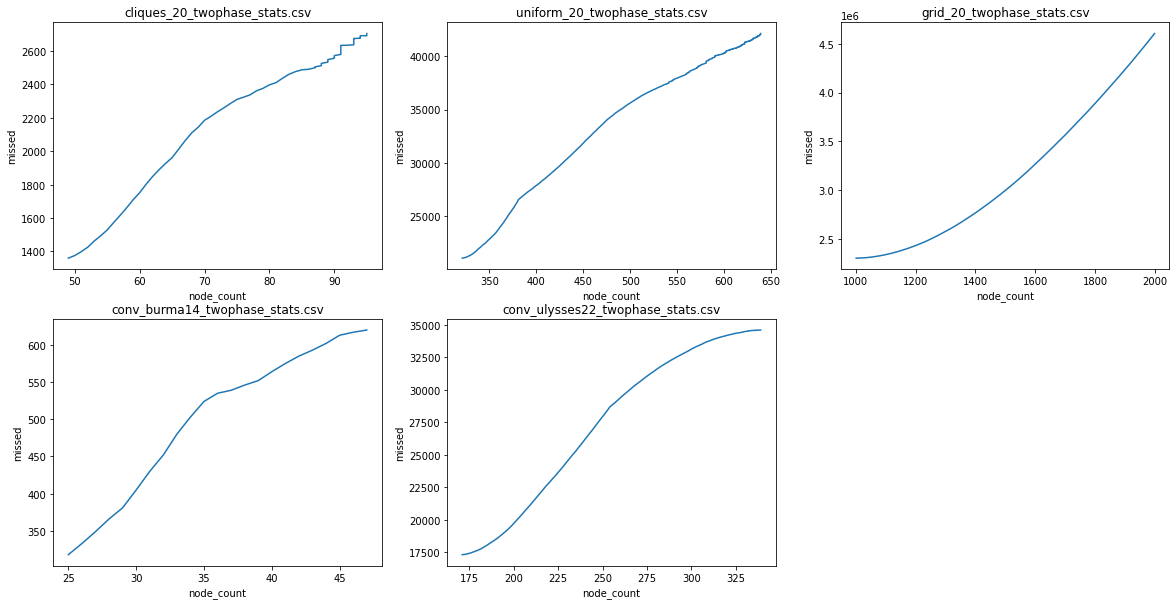
\includegraphics[width=\textwidth]{chapters/experiments/img/merged_plots/per1_all/missed.png}
    \caption{Liczba nieudanych prób tworzenia krawędzi w zależności od liczby wierzchołków --- próbkowanie dwufazowe}
    \label{fig:small_missed}
\end{figure}

\newpage
\foreach \metric/\cap in \metrics{
    \begin{figure}[p]
        \centering
        \includegraphics[width=\textwidth]{chapters/experiments/img/merged_plots/main_snowball/\metric.png}
        \caption{\cap \space w zależności od liczby wierzchołków - próbkowanie snowball}
        \label{fig:main_snowball_\metric}
    \end{figure}
}

\newpage

\foreach \metric/\cap in \metrics{
    \begin{figure}[p]
        \centering
        \includegraphics[width=\textwidth]{chapters/experiments/img/merged_plots/main_twophase/\metric.png}
        \caption{\cap \space w zależności od liczby wierzchołków - próbkowanie dwufazowe}
        \label{fig:main_twophase_\metric}
    \end{figure}
}

\begin{figure}[h!]
    \centering
    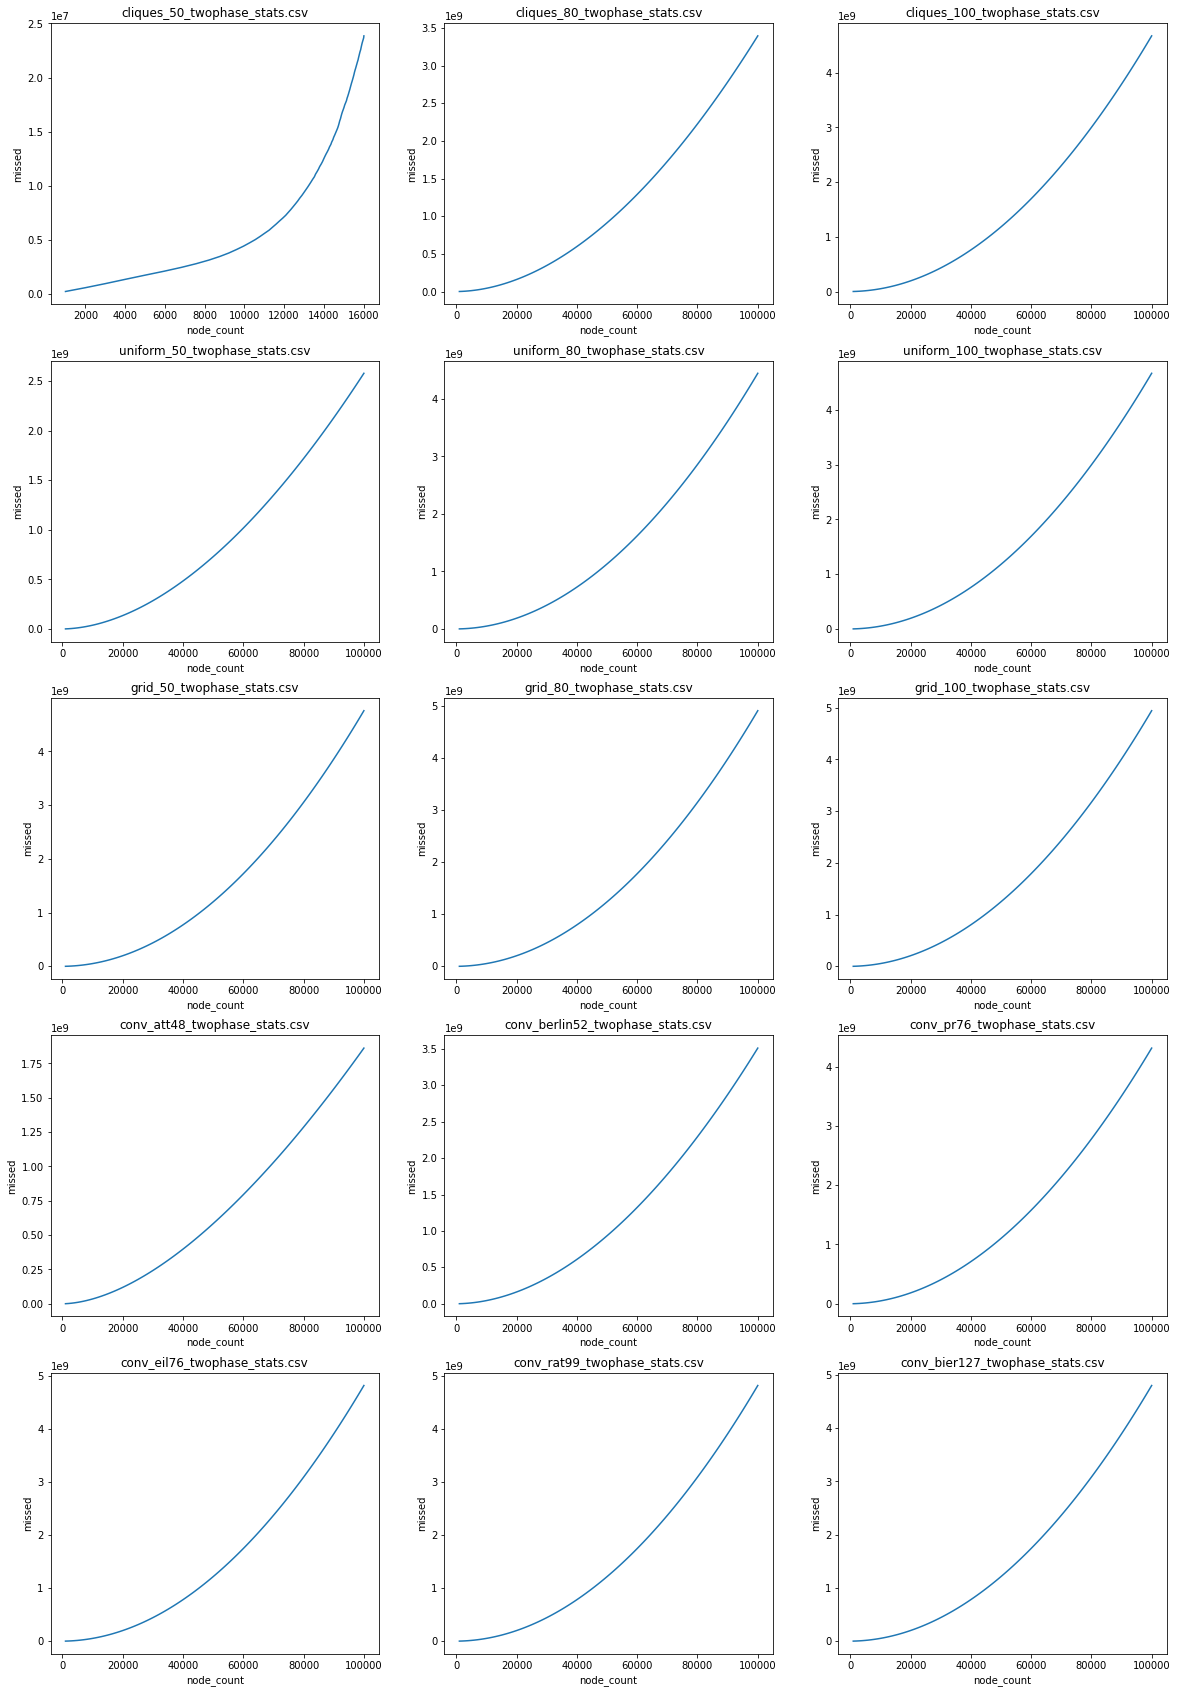
\includegraphics[width=\textwidth]{chapters/experiments/img/merged_plots/main_twophase/missed.png}
    \caption{Liczba nieudanych prób tworzenia krawędzi w zależności od liczby wierzchołków - próbkowanie dwufazowe}
    \label{fig:main_twophase_missed}
\end{figure}

\begin{figure}[h!]
    \centering
    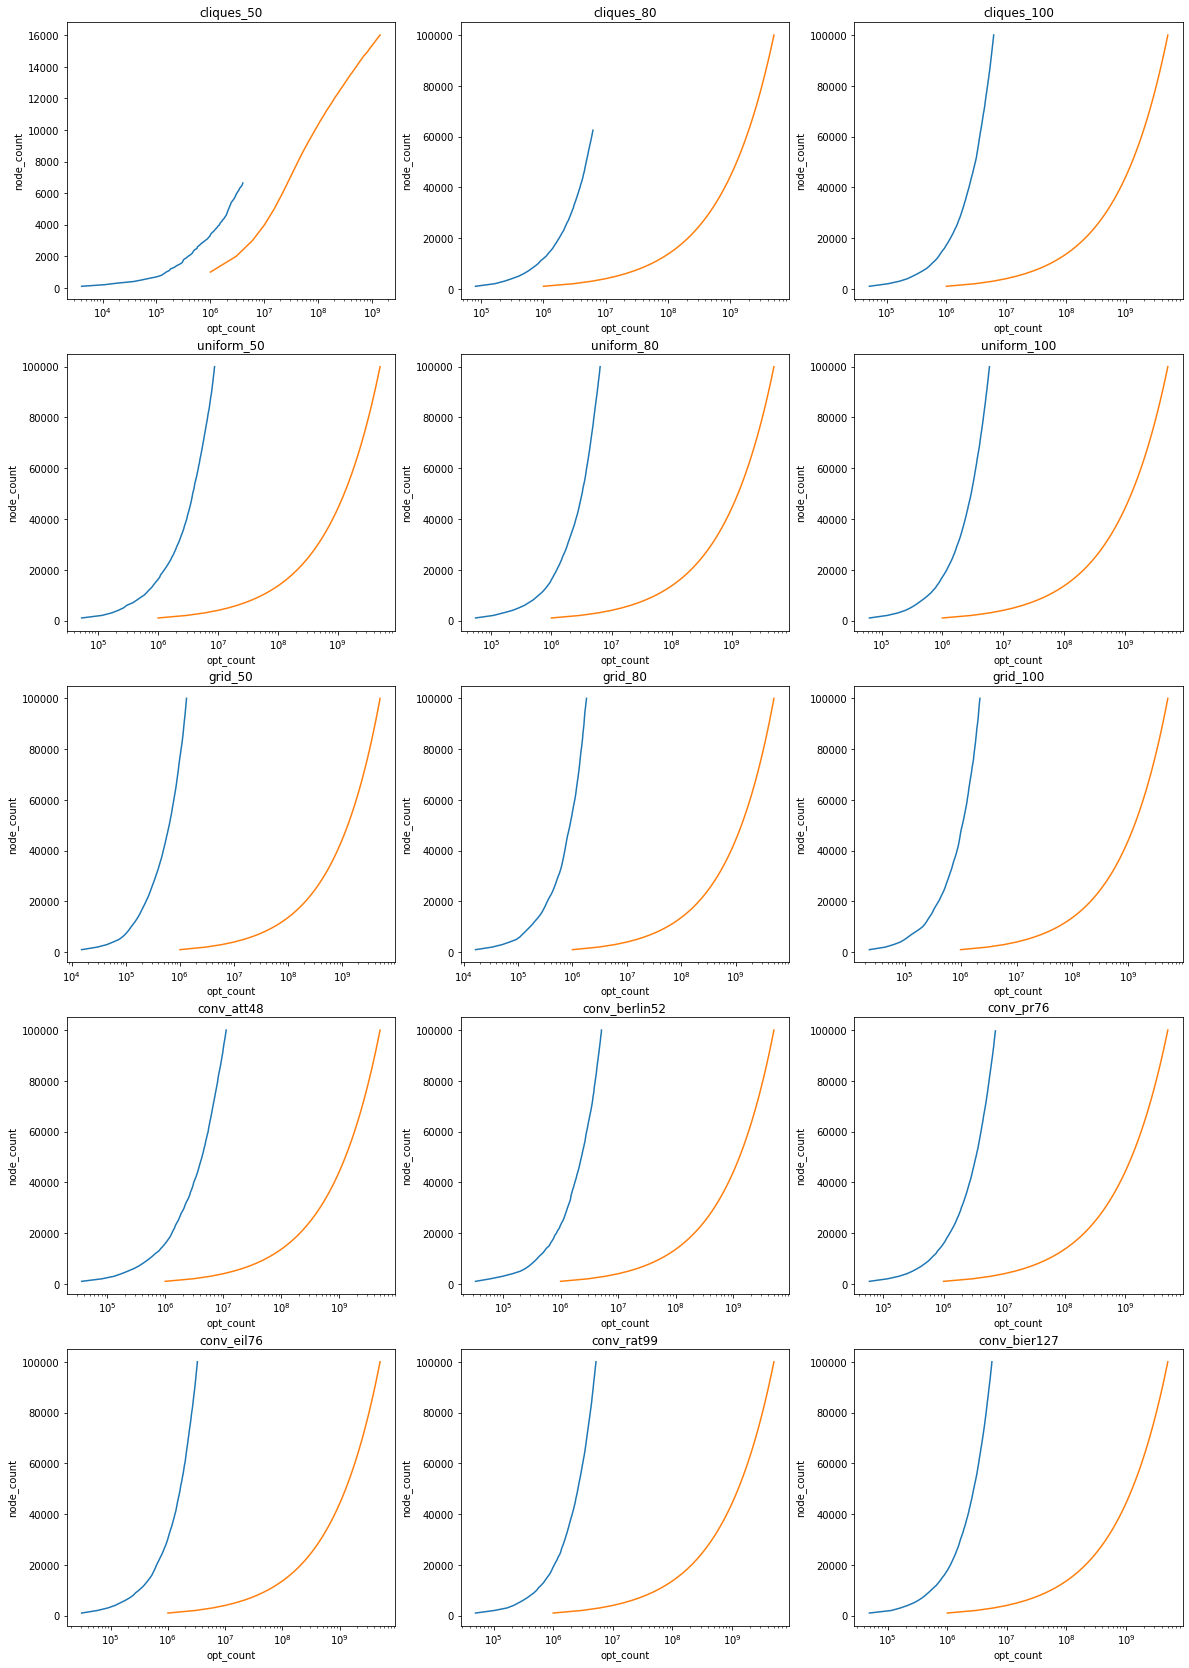
\includegraphics[width=\textwidth]{chapters/experiments/img/opt_nodes.png}
    \caption{Wykres zależności liczby wierzchołków od liczby wywołań funkcji celu.
        Kolor niebieski - próbkowanie snowball, kolor pomarańczowy - próbkowanie dwufazowe.
        Oś X w skali logarytmicznej}
    \label{fig:main_opt_nodes}
\end{figure}

\begin{figure}[h!]
    \centering
    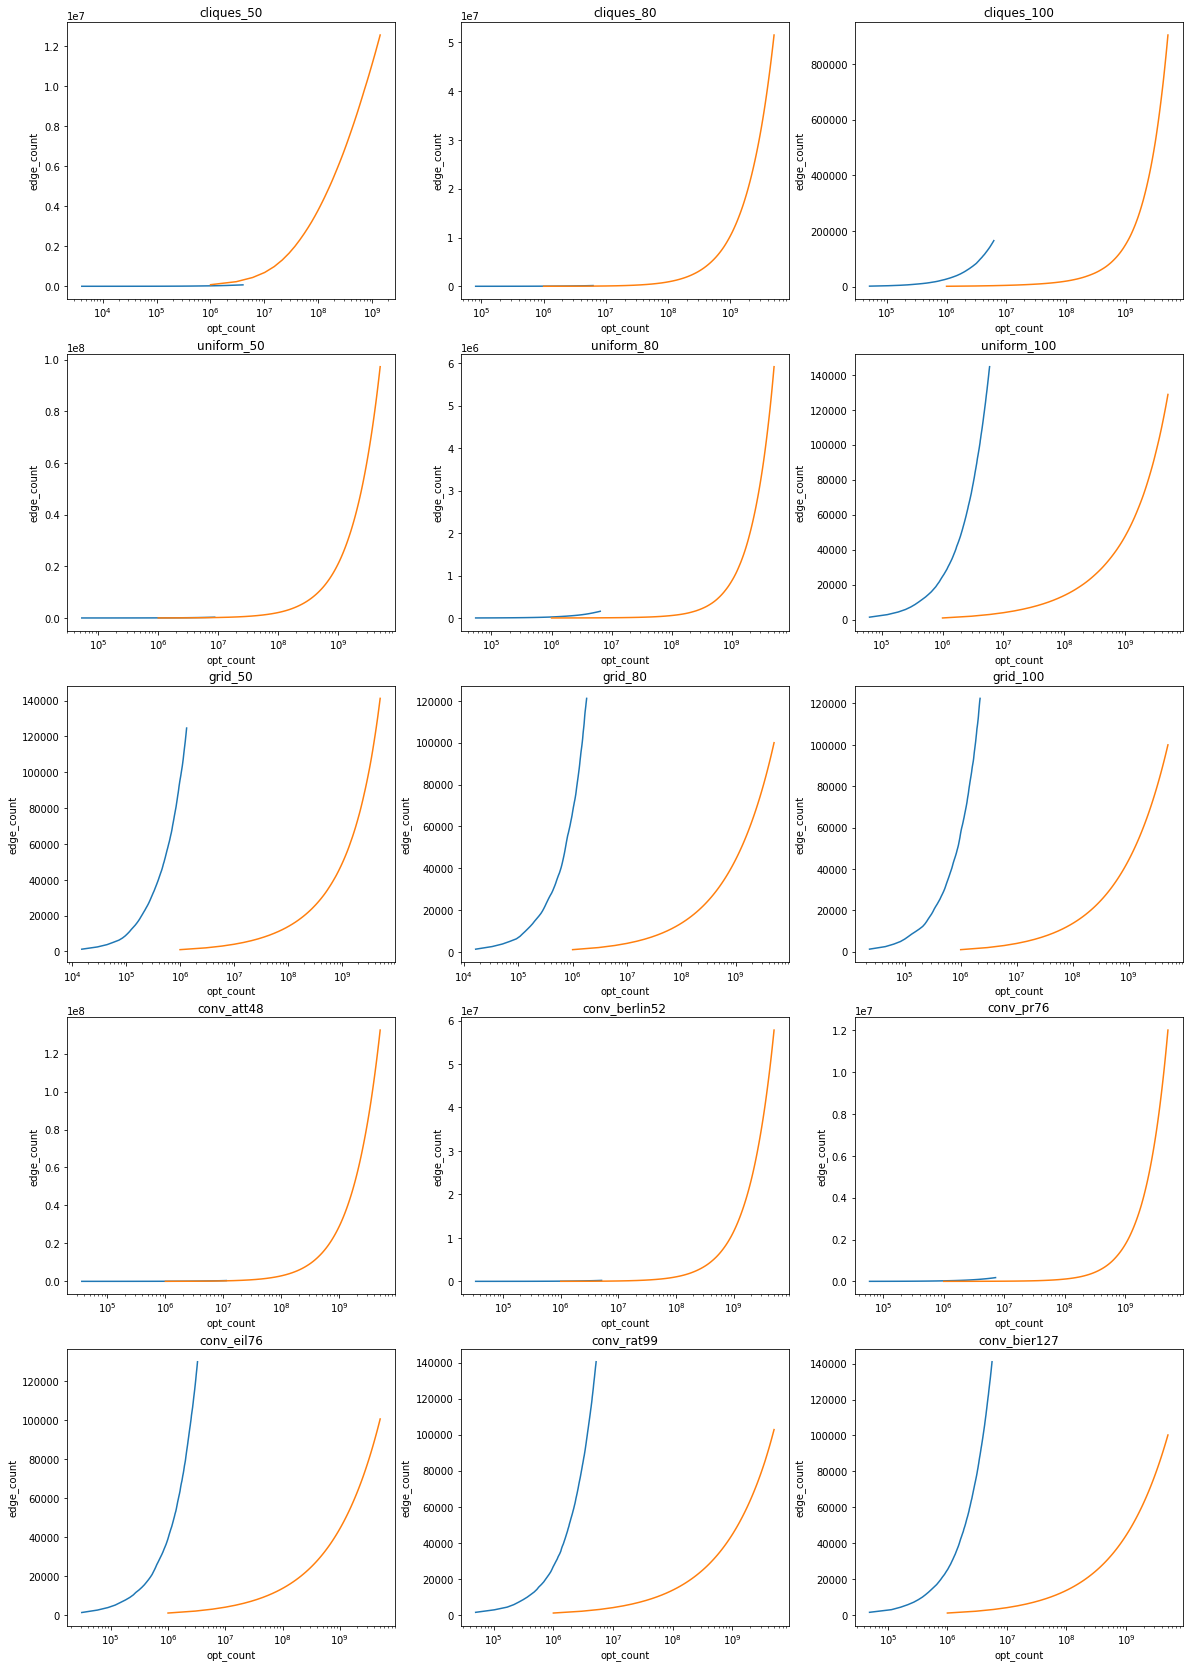
\includegraphics[width=\textwidth]{chapters/experiments/img/opt_edges.png}
    \caption{Wykres zależności liczby krawędzi od liczby wywołań funkcji celu.
        Kolor niebieski - próbkowanie snowball, kolor pomarańczowy - próbkowanie dwufazowe.
        Oś X w skali logarytmicznej}
    \label{fig:main_opt_edges}
\end{figure}


